%----------------------------------------------------------------------------------------
%	MODULE INFORMATION
%----------------------------------------------------------------------------------------

% Define the top matter
\setModuleTitle{Variants visualization}
\setModuleAuthors{%
  Mathieu Bourgey \mailto{mathieu.bourgey@mcgill.ca}%
}
\setModuleContributions{%
}


%----------------------------------------------------------------------------------------
%	MODULE TITLE PAGE
%----------------------------------------------------------------------------------------

\chapter{\moduleTitle}

%----------------------------------------------------------------------------------------

\newpage

%----------------------------------------------------------------------------------------
%	LEARNING OUTCOMES
%----------------------------------------------------------------------------------------

The on-line version is available at here:
\url{https://github.com/mbourgey/EBI_cancer_workshop_visualization/tree/australia_2015}

\section{Key Learning Outcomes}

After completing this practical the trainee should be able to:

\begin{itemize}
  \item Generate circos like graphics using R
\end{itemize}

%----------------------------------------------------------------------------------------
%	MODULE RESOURCES
%----------------------------------------------------------------------------------------

\section{Resources You'll be Using}

\subsection{Tools Used}

\begin{description}[style=multiline,labelindent=0cm,align=left,leftmargin=1cm]
  \item[R] \hfill\\
    \url{https://cran.r-project.org/}
  \item[R package circlize] \hfill\\
    \url{https://cran.r-project.org/web/packages/circlize/index.html}

\end{description}


\newpage

%----------------------------------------------------------------------------------------
%	INTRODUCTION
%----------------------------------------------------------------------------------------

\section{Introduction}

This short workshop will show you how to visualize your data.

We will be working on 3 types of somatic calls: 
\begin{itemize}
  \item SNV calls from MuTect (vcf)
  \item SV calls from DELLY (vcf)
  \item CNV calls from SCoNEs (tsv)
\end{itemize}

This work is licensed under a Creative Commons Attribution-ShareAlike 3.0 Unported License. This means that you are able to copy, share and modify the work, as long as the result is distributed under the same license.



%----------------------------------------------------------------------------------------
%	THE ENVIRONMENT
%----------------------------------------------------------------------------------------

\section{Prepare the Environment}

We will use a dataset derived from the analysis of whole genome sequencing paired normal/tumour samples

The call files are contained in the folder visualization:

\begin{description}[style=multiline,labelindent=1.5cm,align=left,leftmargin=2.5cm]
  \item[\texttt{mutect.somatic.vcf} \hfill\\]
  \item[\texttt{delly.somatic.vcf} \hfill\\]
  \item[\texttt{scones.somatic.tsv} \hfill\\] 
\end{description}




%----------------------------------------------------------------------------------------
%	CIRCULAR REPRESENTATION OF YOUR CALLS
%----------------------------------------------------------------------------------------

Many tools are available to do this the most common know is circos. But circos is a really not user friendly. In this tutoriel we show you an easy alternative to build circular representation of genomic data.

First we need to go in the folder to do the analysis

\begin{steps}
\begin{lstlisting}
cd /home/trainee/visualization/
\end{lstlisting}
\end{steps}

Let see what is in this folder

\begin{steps}
\begin{lstlisting}
ls
\end{lstlisting}
\end{steps}

circos.R delly.somatic.vcf mutect.somatic.vcf scones.somatic.tsv

Take a look of the data files.

These are data of the are not restricted to a short piece of the chromosome.

SNVs have already been filtered 

\begin{steps}
\begin{lstlisting}
less mutect.somatic.tsv
less delly.somatic.vcf
less data/scones.somatic.30k.tsv
\end{lstlisting}
\end{steps}


\begin{questions}
\texttt{What can you see from this data ?}
\end{questions}


\begin{answer}
I saw:
\begin{itemize}
  \item the filtered output of 3 differents software: mutect (SNVs), delly (SVs), SCoNEs (CNVs)
  \item The 3 files show 2 different formats (vcf, tsv)
  \item almost all type of variant are represented here: mutations, deletion, inversion, translocation, large amplification and deletion (CNVs)
\end{itemize}
\end{answer}




\begin{questions}
\texttt{Why don't we use the vcf format for all type of call?}
\end{questions}


\begin{answer}
The 1000 Genomes project try to use/include SVs call in the vcf format. Some tools like Delly use this format for SV. This a good idea to try to include everything altogether but, to my point of view, this not the best way to handle SV and CNV. 

Why ?

Due to the nature of these calls, you can not easily integrate the postional information of the two breakpoints (that could be located faraway or in an other chormosome) using a single position format.
\end{answer}



The analysis will be done using the R program

\begin{steps}
\begin{lstlisting}
R
\end{lstlisting}
\end{steps}

We will use the circlize package from the cran R project. This package is dedicated to generate circular plot and had the advantage to provide pre-build function for genomics data. One of the main advantage of this tools is the use of bed format as input data.

\begin{steps}
\begin{lstlisting}
library(circlize)
\end{lstlisting}
\end{steps}


Let's import the variants

\begin{steps}
\begin{lstlisting}
snp=read.table("mutect.somatic.vcf")
sv=read.table("somatic.sv.vcf")
cnv=read.table("data/scones.somatic.tsv",header=T)
\end{lstlisting}
\end{steps}


We need to set-up the generic graphical parameters

\begin{steps}
\begin{lstlisting}
par(mar = c(1, 1, 1, 1))
circos.par("start.degree" = 90)
circos.par("track.height" = 0.05)
circos.par("canvas.xlim" = c(-1.3, 1.3), "canvas.ylim" = c(-1.3, 1.3))
\end{lstlisting}
\end{steps}

Let's draw hg19 reference ideograms

\begin{steps}
\begin{lstlisting}
circos.initializeWithIdeogram(species = "hg19")
\end{lstlisting}
\end{steps}

Unfortunately circlize does not support hg38 yet. So we will need to reformat our data to fit the hg19 standards
As we work only on autosomes we won't need to lift-over and we could simply add \textbf{chr} at the begin of the chromosome names

We can now draw 1 track for somatic mutations

\begin{steps}
\begin{lstlisting}snv_tmp=read.table("data/mutec.somatic.vcf",comment.char="#")
snv=cbind(paste("chr",as.character(snp[,1]),sep=""),snp[2],snp[,2]+1)
circos.genomicTrackPlotRegion(snv,stack=TRUE, panel.fun = function(region, value, ...) {
    circos.genomicPoints(region, value, cex = 0.05, pch = 9,col='orange' , ...)
})
\end{lstlisting}
\end{steps}


Let's draw the 2 tracks for cnvs. One track for duplication in red and one blue track for deletion.

\begin{steps}
\begin{lstlisting}
dup=cnv[cnv[,5]>2,]
dup[,1]=paste("chr",as.character(dup[,1]),sep="")
del=cnv[cnv[,5]<2,]
del[,1]=paste("chr",as.character(del[,1]),sep="")
circos.genomicTrackPlotRegion(dup, stack = TRUE,panel.fun = function(region, value, ...) {
        circos.genomicRect(region, value, col = "red",bg.border = NA, cex=1 , ...)
})
circos.genomicTrackPlotRegion(del, stack = TRUE,panel.fun = function(region, value, ...) {
        circos.genomicRect(region, value, col = "blue",bg.border = NA, cex=1 , ...)
})
\end{lstlisting}
\end{steps}


We can cleary see a massive deletion in the chromosome 3.

To finish we just need to draw 3 tracks + positional links to represent SVs

Unfortunately the vcf format has not been designed for SVs. SVs are defined by 2 breakpoints and the vcf format store the second one in the info field. So we will need to extract this information to draw these calls.

\begin{steps}
\begin{lstlisting}
chrEnd=NULL
posEnd=NULL
for (i in 1:dim(sv)[1]) {
    addInfo=strsplit(as.character(sv[i,8]),split=";")
    chrInf=strsplit(addInfo[[1]][3],split="=")
    chrEnd=c(chrEnd,chrInf[[1]][2])
    posInf=strsplit(addInfo[[1]][4],split="=")
    posEnd=c(posEnd,posInf[[1]][2])
}
svTable=data.frame(paste("chr",sv[,1],sep=""),as.numeric(sv[,2]),as.numeric(posEnd),paste("chr",chrEnd,sep=""),as.character(sv[,5]))
\end{lstlisting}
\end{steps}

Now that we reformat the SV calls, let's draw them
\begin{steps}
\begin{lstlisting}
typeE=c("<DEL>","<INS>","<INV>")
colE=c("blue","black","green")
for (i in 1:3) { 
        bed_list=svTable[svTable[,5]==typeE[i],]
        circos.genomicTrackPlotRegion(bed_list,stack=TRUE, panel.fun = function(region, value, ...) {
                circos.genomicPoints(region, value, cex = 0.5, pch = 16, col = colE[i], ...)
        })
}

bed1=cbind(svTable[svTable[,5]=="<TRA>",1:2],svTable[svTable[,5]=="<TRA>",2]+5)
bed2=cbind(svTable[svTable[,5]=="<TRA>",c(4,3)],svTable[svTable[,5]=="<TRA>",3]+5)

for (i in 1:dim(bed1)[1]) {
	circos.link(bed1[i,1],bed1[i,2],bed2[i,1],bed2[i,2])
}
\end{lstlisting}
\end{steps}


A good graph needs title and legends

\begin{steps}
\begin{lstlisting}
title("Somatic calls (SNV - SV - CNV)")
legend(0.7,1.4,legend=c("SNV", "CNV-DUPLICATION","CNV-DELETION","SV-DELETION","SV-INSERTION","SV-INVERSION"),col=c("orange","red","blue","blue","black","green","red"),pch=c(16,15,15,16,16,16,16,16),cex=0.75,title="Tracks:",bty='n')
legend(0.6,0.95,legend="SV-TRANSLOCATION",col="black",lty=1,cex=0.75,lwd=1.2,bty='n')
\end{lstlisting}
\end{steps}


you should obtain a plot like this one:
\begin{figure}[h]
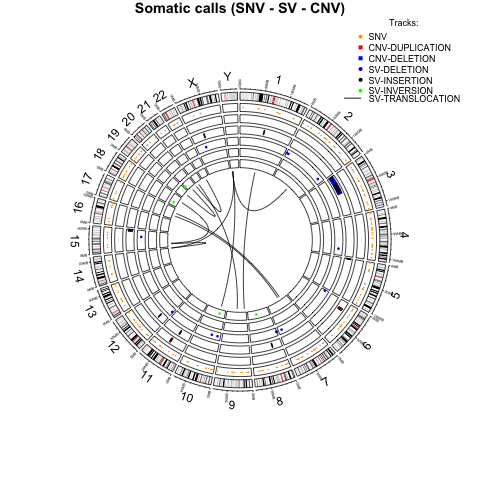
\includegraphics[width=0.5\textwidth]{circos.png}
\end{figure}

\begin{questions}
\texttt{could you generate the graph and save it into a pdf file ?}
\end{questions}

\begin{answer}
\begin{steps}
\begin{lstlisting}
circos.clear()
pdf("circos.pdf")
...
dev.off()
\end{lstlisting}
\end{steps}
\end{answer}

Finally exit R

\begin{steps}
\begin{lstlisting}
q("yes")
\end{lstlisting}
\end{steps}


\newpage

%----------------------------------------------------------------------------------------
%	ACKNOWLEDGEMENTS
%----------------------------------------------------------------------------------------

\section{Acknowledgements}
I would like to thank and acknowledge Louis Letourneau for this help and for sharing his material. The format of the tutorial has been inspired from Mar Gonzalez Porta. I also want to acknowledge Joel Fillon, Louis Letrouneau (again), Francois Lefebvre, Maxime Caron and Guillaume Bourque for the help in building these pipelines and working with all the various datasets.
